\documentclass[TAU.tex]{subfiles}
\begin{document}

\chapter{Математическое описание непрерывных систем уравнений} % (fold)

В ТАУ при анализе и синтезе САУ рассматриваются их {\it математические модели}.
\defi{\it Математическая модель} (ММ) - уравнения, переходные и временные функции, которые описывают процессы, происходящие в САУ.
Существует два способа получения ММ: теоретический и экспериментальный.\par
{\it Теоретический метод} заключается в аналитическом исследовании физической сущности процесса с использованием общих законов физики, или процессов с использованием материального и энергетического баланса. Применение чисто теоретического метода представляет большую трудность вследствие сложности явлений, происходящих в процессах, или недостаточной степени изученности их.
{\it Экспериментальный метод} математического описания заклю­чается в обработке экспериментальных данных, полученных непо­средственно на действующих объектах производства, или на полу­промышленной лабораторной машине, или физической модели про­цесса — стенде.\par
Наиболее эффективным методом получения математической модели является сочетание {\itтеоретического} и {\it экспериментального} ме­тодов. При этом на долю теоретического метода приходится анализ в основном структурных свойств объекта и продуктов и получение общего вида уравнений, а на долю экспериментального — количе­ственный анализ и проверка теоретических выводов.\par
При построении ММ неизбежно возникают противоречивые требования: достаточная точность модели и доступность, или простота, анализа модели. Чем выше точность модели, тем она сложнее; чем проще исследовать ММ, тем она проще. Цель, которую ставит перед собой разработчик или исследователь, разрешает данное противоречие. 




\section{Уравнения динамики и статистики} % (fold)

Любой элемент (часть) САУ осуществляет преобразование входа $g$ (или $u$) в выход $y$:
$$
y(t) = A g(t),
$$
где $A$ --- оператор САУ. В этом курсе мы будем рассматривать только оператор $A$, описываемый обыкновенными дифференциальными уравнениями (ОДУ). Введем два вида уравнений, рассматриваемых в ТАУ.

\defi{\it Уравнение статистики} - уравнение, описывающее статический (установившийся) режим.
\defi {\it Уравнение динамики} - уравнение, описывающее процесс в звене при произвольных входных воздействиях.

Пусть дано ОДУ некоторого ОУ вида
\begin{equation}\label{EQ_DYNAMIC}
F(y,\dot y, \ddot y, u, \dot u, v) = 0,
\end{equation}
где $F$ --- функция нескольких переменных, $y$ и $u$ --- выход и управление, $v$ --- возмущение.

Пусть при $u=u^0$ и $v=v^0$ со временем выход $y$ принимает постоянное значение: $y=y^0$. Тогда уравнение \eref{EQ_DYNAMIC} примет вид
\begin{equation}\label{EQ_STATIC}
F^0=F(y^0, 0, 0, u^0, 0, v^0) = 0.
\end{equation}
Уравнение \eref{EQ_STATIC} называется уравнением статики, уравнение \eref{EQ_DYNAMIC} называют уравнением динамики.

\subsection{Звено САУ} % (fold)

\defi{\it Звеном} называют ММ либо части САУ, либо САУ целиком. Понятие звена удобно использовать для представления САУ в виде соединения нескольких звеньев, т.е. более простых ММ.

Одно из самых простых звеньев - это усилитель, П[ропорциональное]-звено. Его уравнение можно записать в виде
$$
y = ku.
$$
Уравнение динамики здесь совпадает с уравнением статики (точнее, динамики просто нет). Такого рода преобразования часто обозначают графически в виде блока.


\begin{figure}[h]
\centering
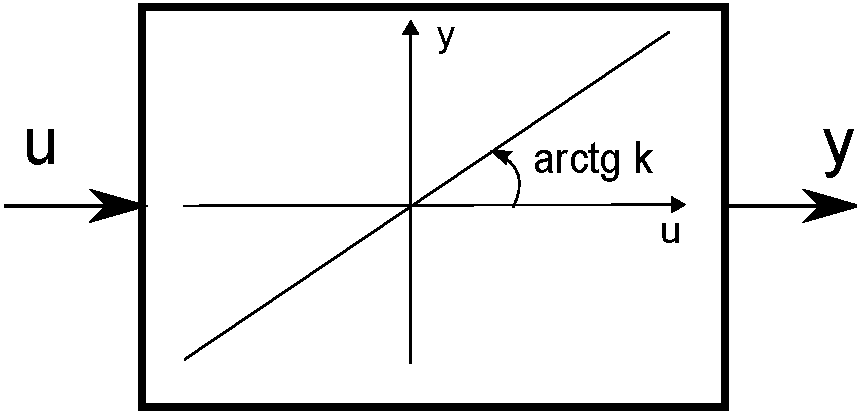
\includegraphics[width=8cm]{block_gain.pdf}
\caption{Статическая характеристика П-звена}
\centering
\end{figure}


% subsection звено_сау (end)

\subsection{Линеаризация} % (fold)

Назначение САУ - это поддержание определенного заданного режима. Поэтому параметры, описывающие САУ, не должны сильно отличаться от заданного режима. Эта простая идея обычно позволяет проводить операцию линеаризации.

\defi{\it Линеаризация} - построение приближенной линейной модели на основе более реалистичной нелинейной модели.

Рассмотрим пример для уравнения \eref{EQ_DYNAMIC}.

Пусть заданный режим имеет вид
$$
y = y^0, \dot y = \ddot y = 0, u=u^0, \dot u = 0, v=v^0.
$$
Тогда реальные параметры САУ можно записать в отклонениях как
$$
y = y^0+\Delta y,\;\dot y = \dot{\Delta y},\;\ddot y = \ddot{\Delta y},\; u = u^0 + \Delta u,\; \dot u = \dot{\Delta u},\;v = v^0 + \Delta v,
$$
где переменные со знаком $\Delta$ достаточно малы.

Тогда для функции $F(y,\dot y, \ddot y, u, \dot u, v)$ воспользуемся разложением в ряд Тейлора в точке $(y^0, 0,0, u^0, 0, v^0)$:
\begin{multline}
F(y,\dot y, \ddot y, u, \dot u, v) = F^0 + \frac{\partial F}{\partial y} \Delta y +\frac{\partial F}{\partial \dot y} \dot{\Delta y}+ \frac{\partial F}{\partial \ddot y} \ddot{\Delta y} +\\  + \frac{\partial F}{\partial u} \Delta u + \frac{\partial F}{\partial \dot u } \dot{\Delta u} + \frac{\partial F}{\partial v} \Delta v + \ldots,
\end{multline}

где $F^0= 0$, многоточием обозначены члены с более высоким порядком малости.

Отсюда получают линеаризацию уравнения \eref{EQ_DYNAMIC} вида

\begin{equation}\label{EQ_LINEAR}
a_2\ddot{\Delta y} + a_1 \dot{\Delta y} + a_0 \Delta y - b_1\dot{\Delta u} - b_0\Delta u - c_0 \Delta v = 0,
\end{equation}

где $a_0 = \frac{\partial F}{\partial y}$, $a_1 = \frac{\partial F}{\partial \dot y}$, $a_2 = \frac{\partial F}{\partial \ddot y}$, $b_0 = -\frac{\partial F}{\partial u}$, $b_1 = -\frac{\partial F}{\partial \dot u }$ и $c_0 = -\frac{\partial F}{\partial v}$.

Введем оператор дифференцирования: $s = \frac{d}{dt}$.

Тогда уравнение \eref{EQ_LINEAR} примет вид (знаки $\Delta$ опущены)
$$
a_2 s^2 y + a_1 s y + a_0 y = b_1 s u + b_0 u + c_0 v,
$$
что эквивалентно
$$
Q(s) y = R_1(s)u + R_2(s)v,
$$
где $Q(s) = a_2s^2 + a_1 s + a_0$ называют {\it собственным оператором}, а $R_1(s) = b_1s+b_0$ и $R_2(s) = c_0$ --- {\it операторами воздействия}.

\defi{\it Собственный оператор} - дифференциальный оператор $Q(s)$ при выходной величине.

\defi{\it Оператор воздействия} - дифференциальный оператор $R(s)$ при входной величине.


% subsection линеаризация (end)

% section уравнения_динамики_и_статистики (end)

\section{Преобразование Лапласа} % (fold)


\subsection{Обратное преобразование Лапласа} % (fold)

% subsection обратное_преобразование_лапласа (end)

\subsection{Свойства преобразования Лапласа и примеры} % (fold)

% subsection свойства_преобразования_лапласа_и_примеры (end)

\subsection{Передаточная функция в изображениях Лапласа} % (fold)

% subsection передаточная_функция_в_изображениях_лапласа (end)

\subsection{Передаточная функция в операторной форме} % (fold)

% subsection передаточная_функция_в_операторной_форме (end)

\subsection{Временные функции} % (fold)

% subsection временные_функции (end)

\subsection{Временные функции} % (fold)

% subsection временные_функции (end)

% section преобразование_лапласа (end)

\section{Частотные функции} % (fold)

% section частотные_функции (end)

\section{Основные типы элементарных звеньев} % (fold)


\subsection{Пропорциональное звено} % (fold)

% subsection пропорциональное_звено (end)

\subsection{Дифференциальное звено} % (fold)

% subsection дифференциальное_звено (end)

\subsection{Интегрирующее звено} % (fold)

% subsection интегрирующее_звено (end)

\subsection{Апериодическое звено} % (fold)

% subsection апериодическое_звено (end)

\subsection{Колебательное звено} % (fold)

% subsection колебательное_звено (end)

\subsection{Звено чистого запаздывания} % (fold)

% subsection звено_чистого_запаздывания (end)

% section основные_типы_элементарных_звеньев (end)

%chapter математическое_описание_непрерывных_систем_уравнений (end)
\end{document}